\chapter{Resultados}
\label{ch:resultados}

% No continuar a la siguiente parte hasta no haber terminado la anterior

%! Mínimo 10 paginas.


%! Revisar
En el siguiente capitulo se van a comentar los diversos resultados obtenidos en el presente TFG, tanto los relacionados con la \emph{FPGA} (\emph{Hardware} usado, simulaciones y sintetizado final), como con el \emph{Software} de control. Se incluyen además, varias imágenes que complementen las explicaciones del mismo.

%! Revisar
\section{Resultados de los elementos \emph{hardware} del sistema.}
Partiendo del esquema dado de analizadores USB \emph{hardware} (figura \ref{fig:esquema-hardware}), se aprecian dos partes implicadas en la captura, por un lado el encargado de capturar la trama, y por otro, el encargado de controlar dicha captura y almacenar los resultados. En esta sección se van a comentar los resultados de la primera de ellas.

\begin{figure}[htb]
    \centering
    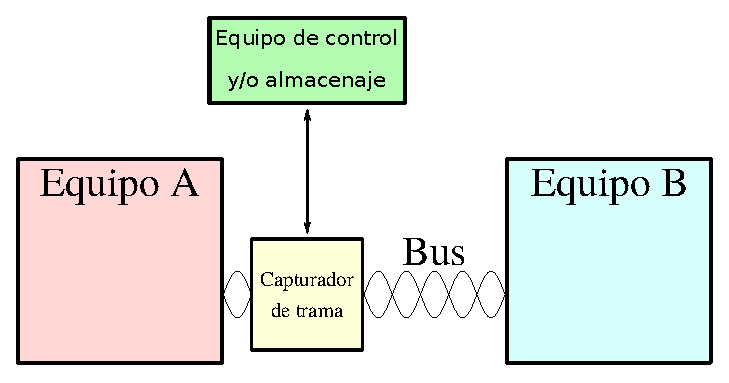
\includegraphics[width=70mm]{esquemas/esquema-captura-hardware-2.eps}
    \caption{Esquema de analizadores \emph{hardware}}
    \label{fig:esquema-hardware}
\end{figure}

%! Revisar
\subsection{Componentes utilizados.}
% ICEStick, USB3300, 3D, cables, etc... Imagen general.

En al figura \ref{fig:sistema_final} se muestra el resultado \emph{hardware} del presente trabajo, este a su vez, está formado por los siguiente componentes.

\begin{figure}[htbp]
    \centering
    \includegraphics[height=110mm]{hw_final/final.jpg}
    \caption{Sistema de captura final}
    \label{fig:sistema_final}
\end{figure}

\begin{enumerate}
    %! Revisar
    \item \textbf{Placa de desarrollo \emph{IceStick \cite{icestickmanual}} (Véase figura~\ref{fig:IceStick_board}).} \\
    Se trata de una placa de desarrollo, que incorpora, sin contar con todos los conectores, indicadores \emph{LEDs}, elementos pasivos y componentes de regulación, la \emph{FPGA iCE40HX-1k \cite{lattice:ice40}} del fabricante \emph{Lattice} \footnote{Página web del producto: \url{https://www.latticesemi.com/Products/FPGAandCPLD/iCE40.aspx}}, memoria SPI de $32MBit$ para almacenar el sintetizado generado, conversor USB a doble puerto de comunicación FIFO \emph{FTDI 2232H \cite{FTDI:FT2232HL}} para comunicarse con el PC y oscilador de $12MHz$ con el que referenciar ciertas partes del circuito.
    
    \begin{figure}[htbp]
        \centering
        \includegraphics[width=125mm]{hw_final/IceStick_board.jpg}
        \caption{Placa de desarrollo \emph{IceStick}}
        \label{fig:IceStick_board}
    \end{figure}

    %! Revisar
    \item \textbf{Módulo encargado de la capa física USB.} \\
    PCB que incorpora el circuito integrado \emph{USB3300 \cite{icestickmanual}} del fabricante \emph{Microchip}. Este se encarga de manejar la capa física del bus USB, comunicándose con la \emph{FPGA} por medio del protocolo \emph{ULPI} \cite{ulpi-specs}. \\
    En al figura \ref{fig:USB3300_board}, se aprecia que dicha \emph{PCB} incluye dos conectores USB, uno tipo A hembra, y otro tipo mini-B hembra. Sus señales de datos están interconectadas, por lo que es en este punto donde ambos extremos del bus a analizar se unen, pudiendo capturar la trama sin interrumpir la conexión debido a que el integrado \emph{USB3300} se puede configurar para mantener sus patillas de datos en alta impedancia.

    \begin{figure}[htbp]
        \centering
        \includegraphics[width=50mm]{hw_final/USB3300_board.jpg}
        \caption{PCB con el integrado \emph{USB3300}}
        \label{fig:USB3300_board}
    \end{figure}

    %! Revisar
    \item \textbf{Cableado de unión (Figura~\ref{fig:matriz-hw-resto:cables}).} \\
    Para conexionar ambas placas, se utilizan varios cables entre el conector del módulo con el integrado \emph{USB3300} y los conectores laterales de la placa \emph{IceStick}. \\
    La \emph{FPGA iCE40HX-1k} posee 4 bancos de señales de entrada/salida, para evitar posibles retrasos en las señales \cite{fpga:routing}, los 8bits de datos paralelos se conectan al banco 0 (pines del 112 al 119), mientras que el resto de señales \emph{ULPI} (DIR, STP, RST y NXT) al banco 2.

    %! Revisar
    \item \textbf{Pulsadores externos (Figura~\ref{fig:matriz-hw-resto:botones}).} \\
    Se han incluido dos botones auxiliares externos, con los que poder tanto reiniciar el sistema en su totalidad, como enviar un \emph{byte} de prueba por el puerto serie. \\
    Las señales son activas a nivel bajo, por lo que se mantienen siempre a nivel alto por medio de unas resistencias de \emph{Pull-Up} (Figura~\ref{fig:buttons_circuit}).

    \begin{figure}[h]
        \centering
        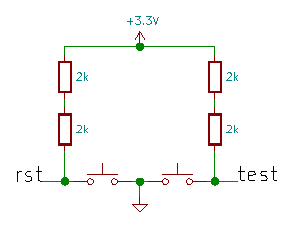
\includegraphics[width=50mm]{hw_final/buttons_circuit2.eps}
        \caption{Esquema de los botones auxiliares}
        \label{fig:buttons_circuit}
    \end{figure}

    %! Revisar
    \item \textbf{Base impresa en 3D (Figura~\ref{fig:matriz-hw-resto:base}).} \\
    Para facilitar el trabajo, se ha diseñado e impreso una pequeña base en 3D, en la cual tener las dos placas unidas y organizadas.

    \begin{figure}[htbp]
        \centering
        \subfigure[Cables de interconexión]{
            \includegraphics[height=40mm]{hw_final/cables.jpg}
            \label{fig:matriz-hw-resto:cables}
        }
        \subfigure[Botones auxiliares]{
            \includegraphics[height=40mm]{hw_final/buttons.jpg}
            \label{fig:matriz-hw-resto:botones}
        } \\
        \subfigure[Base 3D]{
            \includegraphics[height=75mm]{hw_final/3D_base.jpg}
            \label{fig:matriz-hw-resto:base}
        }
        \caption{Resto de elementos usados en el sistema de captación} 
        \label{fig:matriz-hw-resto}
    \end{figure}
\end{enumerate}


%! Revisar [Añadir algo mas??]
\subsection{Lista de funcionalidades integradas en la \emph{FPGA}.}
% Módulo Puerto serie a X baudios (shift register, clk_baud, etc...), ULPI, FIFO, etc... 
Se han diseñado e implementado las siguientes funcionalidades.

\begin{itemize}
    %! Revisar
    \item \textbf{Sistema de comunicación serie.} \\
    Sistema capaz de generar señales compatibles con una comunicación bidireccional serie 8N1 \footnote{8N1: $8~bits$ de datos, sin $bit$ de paridad y un $bit$ de parada}, consiguiendo una tasa de transferencia estable máxima de $3750000~bauds$. A su vez, tanto para la lectura coma para la escritura, se hah incorporado unos \emph{buffers} de $512~bytes$ cada uno.
    
    %! Revisar
    \item \textbf{Sistema de comunicación \textit{ULPI}.} \\
    Sistema, que de forma síncrona al reloj de $60MHz$ generado por el integrado \emph{USB3300}, sea capaz tanto de procesar como de generar señales \textit{ULPI} tal como se contempla en su especificación \cite{ulpi-specs}. \\
    De todos los modos de funcionamiento de dicho bus, y tal como se ha comentado en el capitulo de \ref{ch:objetivos}, se han creado los modos encargados de leer y escribir registros, y el modo de recibir datos USB.
    
    %! Revisar
    \item \textbf{Protocolo básico de control entre el sistema de captura y el PC.} \\
    Diseño e implementación de un simple protocolo, que haciendo uso del sistema de comunicación serie, sea capaz de controlar el sistema y recibir los datos USB capturados. \\
    Siempre que se desee ejecutar un comando en el sistema de captura, el PC envía $2~bytes$ (\emph{YYZZZZZZ\_XXXXXXXX}), separados a su vez en tres grupos, de 2, 6 y 8 $bits$ respectivamente. Tal como se recoge en la tabla \ref{tab:comandos_operacion}, el primer grupo indica que comando se debe realizar, el segundo la dirección en la que realizar dicha operación, y el tercero, los datos a utilizar.

    \begin{table}[htbp]
        \caption{Información de los $bytes$ enviados a la \emph{FPGA}.}
        \centering
        \label{tab:comandos_operacion}
        \begin{tabular}{|c|c|c|c|c|}
            \hline
            % Bits operación ($2~bits$) & Bits dirección ($6~bits$) & Bits datos ($8~bits$) & Descripción                                    & Respuesta \\ \hline
            Bits comando & Bits dirección & Bits datos & Descripción & Respuesta \\ \hline
            \hline
            00 & Indiferente & 10010110 & \begin{tabular}{@{}c@{}}Activar/desactivar \\ envío de datos USB\end{tabular} & --       \\ \hline
            01 & Indiferente & Indiferente & \begin{tabular}{@{}c@{}}Enviar último valor \\ de registro leído\end{tabular} & 1 byte   \\ \hline
            10 & Dirección a escribir & Datos a escribir & Escribir registro \emph{ULPI} & -- \\ \hline
            11 & Dirección a leer & Indiferente & Leer registro \emph{ULPI} & --              \\ \hline
        \end{tabular}
    \end{table}

    %! Revisar
    \item \textbf{Memoria de almacenamiento temporal.} \\
    Debido a que los datos USB son capturados a una velocidad muy superior a la velocidad máxima de transmisión del puerto serie, se debe implementar una memoria en la que poder almacenarlos temporalmente. Para ello, se hace uso de varios de los bloques de memoria \emph{RAM} incorporados en la propia \emph{FPGA}, consiguiendo $4~KBits$.
    % Debe evitarse la perdida de los datos USB capturados, ya que dicha informacion es recogida a una velocidad mayor, por lo tanto, se almacenan temporalmente
\end{itemize}

%! Añadir mas [Fotos??]
\subsection{Simulaciones finales.}
% Partes de la simulación, imagen de GTKwave, resultados de la simulación, etc...
Con el objetivo de eliminar posibles errores capaces de dañar los propios componentes \emph{hardware}, y para comprobar el correcto funcionamiento del sistema, se han realizado diversas pruebas previas al sintetizado y utilización de la configuración final. \\
Estás pruebas, tal como está explicado en el capítulo de procedimientos (Capítulo~\ref{ch:procedimiento}), hacen uso de las herramientas de código abierto \emph{Icarus Verilog}\footnote{Véase su repositorio: \url{https://github.com/steveicarus/iverilog}}, encargada de simular el propio código de \emph{Verilog}, y el visor de ondas \emph{GTKWave}, permitiendo generar y mostrar gráficamente todas las señales del circuito en cualquier instante de tiempo.

%! Revisar
Se ha dividido la simulación en las siguiente pruebas:
\begin{enumerate}
    %! Revisar
    \item \textbf{Pruebas de botones auxiliares.}
    Se simulan las pulsaciones de los botones externos de la \emph{FPGA}, produciendo un reinicio con el primero, y un envío de un $byte$ por el puerto serie con el segundo.

    %! Revisar
    \item \textbf{Prueba de lectura de registro.}
    Se simula una petición enviada por el puerto serie, que realice una lectura de registro \emph{ULPI}.
    
    %! Revisar
    \item \textbf{Prueba de transmisión del último registro leído.}
    Se simula una petición enviada por el puerto serie para enviar el valor del registro anteriormente leído al PC.
    
    %! Revisar
    \item \textbf{Prueba de escritura de registro.}
    Se simula una petición enviada por el puerto serie, que escriba un $byte$ en un registro del integrado \emph{USB3300}.
    
    %! Revisar
    \item \textbf{Prueba de captación de 6 bytes \noWord[Añadir símbolo] USB.}{\label{enum:captacion_6}}
    Prueba en la que se simula la llegada de $6~bytes$ de datos USB, se comprueba también el correcto guardado de los mismos en la memoria interna de la \emph{FPGA}.
    
    %! Revisar
    \item \textbf{Prueba de activación de la transmisión de datos capturados.}{\label{enum:activacion_transmision}}
    Se simula una petición enviada por el puerto serie, con la que activar el envío automático de los datos capturados.
    
    %! Revisar
    \item \textbf{Prueba de captación de 4 bytes USB.}
    De igual manera que la prueba \ref{enum:captacion_6}, pero enviando esta vez $4~bytes$ con el envio de datos al PC activado.
    
    %! Revisar
    \item \textbf{Prueba de captación de cambios de estado del bus USB.}
    Se simula un cambio de estado USB enviado por el bus \emph{ULPI}, observando si se actualiza en la \emph{FPGA}.
    
    %! Revisar
    \item \textbf{Prueba de finalización de la transmisión de datos capturados.}
    De igual manera que en la prueba \ref{enum:activacion_transmision} se activaba el envió de datos automático, se realiza la misma petición, desactivandolo en este caso.
\end{enumerate}


%!
\subsection{Información del sintetizado final.}
% No se me ocurre nada ahora. Peso archivo, baudios, etc... Modos de generacion sisnttizado
Tras la finalización de todos los módulos necesarios en \emph{Verilog}, simulando el proyecto en su totalidad, ya se dispondr
Con los modulos generados, y las simulacione realizadas, se dispone de una 
\begin{itemize}
    \item \emph{Yosys.} Herramienta
    \item \emph{Project IceStorm tools}
    \item \emph{Nextpnr}
\end{itemize}
\begin{itemize}
    \item 
\end{itemize}


%!
\section{Resultados del \emph{software} de control y guardado.}
% Pequeña intro de la App, Linux, etc...
A medida que se ha ido desarrollando la parte \emph{hardware}, se han creado pequeñas utilidades 


\noWord[Comentar más de esta frase, ya que la utilizo mas adelante] El sistema en su conjunto no sería funcional, sin una aplicación que utilice los recursos creados para recibir y almacenar la captura.



%! Revisar
\subsection{Aplicaciones de utilidad.}
% lenguaje, hilos, librerías, etc...
A medida que se ha ido desarrollando la parte \emph{hardware}, se han creado varias utilidades en lenguaje \emph{Python}, con las que realizar cálculos de forma rápida o con las que comprobar el funcionamiento de ciertas partes del sistema. Hay que destacar:
\begin{enumerate}
    %! Revisar
    \item \textbf{Utilidad de divisiones del reloj.} \\
    Utilidad con la que poder realizar de forma rápida varios cálculos relacionados con los relojes de entrada. Por ejemplo, obtener los valores óptimos con los que dividir un reloj para generar unos baudios deseados. En el listado \ref{src:utilidad_divisiones_reloj_out}, se plasma un ejemplo de uso.
    \begin{lstlisting}[language=bash,
        caption={Ejemplo de la utilidad de divisiones de reloj.},
        label=src:utilidad_divisiones_reloj_out]
$ ./get_divider.py
  Usage: ./get_divider.py [option] arg1 arg2
  Options: 
      -o: Print the optimal counter value for a given clock (arg1) and Serial baudrate (arg2). [Default]
      -b: Print the minimal divider value for a given clock (arg1) and Serial baudrate (arg2).
      -d: Print the minimal divider value for a given clock (arg1) and time (arg2).
      -t: Print the time (and serial baudrate) for a given clock (arg1) and divider (arg2).
      -a: Print, for a given clock (arg1), all the possible periods that can be generated between 0 and arg2.
      -c: Print the clock for a given time (arg1) and divider (arg2).
$ ./get_divider.py -o 12000000 115200
  Optimal counter value: 105
$ ./get_divider.py -b 12000000 9600
  Recomended divider (with 18% error): 10 [8.533333333333334e-05s]
  10 [8.533333333333334e-05s] - [0.00010416666666666667s] - 11 [0.00017066666666666668s]          
    \end{lstlisting}
    
    %! Revisar
    \item \textbf{Utilidad de generación de baudios.} \\
    Pequeña aplicación que, para los $baudios$ más comunes, genere varias definiciones de \emph{Verilog} a usar por el módulo encargado de generar el reloj del puerto serie. En el listado \ref{src:utilidad_baudios_out} se muestra un ejemplo de la salida de la aplicación.
    \\ \noWord[Borrar listado??? La verdad, es algo inutil ponerlo]
    \begin{lstlisting}[language=bash,
        caption={Ejemplo de la utilidad de generación de baudios ante \emph{60 MHz} de entrada.},
        label=src:utilidad_baudios_out]
$ ./gen_bauds.py
  `define B921600 66
  `define B460800 131
  `define B256000 235
  `define B230400 261
  `define B153600 391
  `define B128000 469
  `define B115200 521
  `define B57600  1042
  `define B56000  1072
  `define B38400  1563
  `define B28800  2084
  `define B19200  3125
  `define B14400  4167
  `define B9600   6250
  `define B4800   12500
  `define B2400   25000
  `define B1200   50000
  `define B600    100000
  `define B300    200000
  `define B110    545455
    \end{lstlisting}
    
    %! Revisar
    \item \textbf{Utilidad de control serie.} \\
    Aplicación, que usando la librería encargada de controlar puertos serie, compruebe el funcionamiento del protocolo. Se puede configurar para abrir el puerto serie a cualquier velocidad, y poder enviar comandos de prueba.
\end{enumerate}

%!
\subsection{Información de la aplicación.}
% lenguaje, hilos, librerías, etc...
Tal como se ha comentado al principio de esta sección, aun teniendo mayor carga la parte \emph{hardware}, es esencial implementar una aplicación que se comunique con ella y permita su funcionamiento. \\
Para ello, utilizando lenguaje C, se ha creado una aplicación, que dando opciones de cntrol con un simple menú, sea capaz de enviar comandos o recibir datos USB. A su vez, es capaz de almacenarlos para su posterior uso o estudio.

La aplicación se ha dividido de la siguiente manera:
\begin{enumerate}
    %!
    \item \textbf{Hilo encargado de controlar las entradas de usuario.} \\
    Tanto la configuración a usar para conectarse a la \emph{FPGA}, como los comandos a enviar 
    a través de un simple menú.

    Tanto la configuración (puerto serie y baudios) usada para conectarse a la \emph{FPGA}, como las posibles peticiones a realizar, se introducen a través de un simple menú

    \begin{lstlisting}[language=bash,
        caption={Ejemplo de la utilidad de generación de baudios ante \emph{60 MHz} de entrada.},
        label=src:utilidad_baudios_out]
$ .sddf
    \end{lstlisting}


    
    %!
    \item \textbf{Hilo encargado de gestionar la comunicación con la \emph{FPGA}, así como almacenar la trama capturada.}
\end{enumerate}


%!
\subsection{Funcionamiento de la aplicación.}
% Imagen del menú, submenus, ejemplo de funcionamiento, etc...

%!
\subsection{Información del archivo generado.}
% Info JSON, como interpretarlo, imagen de ejemplo, etc...
Los dato


% Ejemplo lectura registro??
% Ejemplo escritura registor??
% Ejemplo captura datos usb??
% Manual de utilización
% Significado de las luces en parte hardware






% ###

% % Partes HW con fotos
% % luego todo el conjunto

% %!
% \section{Resultados de los elementos \emph{hardware} del sistema.}


% %!
% \subsection{Componentes \emph{Hardware} utilizados.}

% % \begin{figure}[htb]
% %     \centering
% %     \includegraphics[width=125mm]{hw_final/final.jpg}
% %     \caption{Placa de desarrollo \emph{IceStick}}
% %     \label{fig:IceStick_board}
% % \end{figure}

% El sistema final del analizador USB está compuesto de las siguientes partes.
% % \begin{enumerate}
%     % %! Revisar
%     % \item \textbf{Placa de desarrollo \emph{IceStick \cite{icestickmanual}}.} \\
%     % Tal como se ve en la figura \ref{fig:IceStick_board}, se trata de una placa de desarrollo que incorpora, sin contar con todos los conectores, indicadores \emph{LEDs}, elementos pasivos y componentes de regulación, la \emph{FPGA iCE40HX-1k \cite{lattice:ice40}} del fabricante \emph{Lattice} \footnote{Página web del producto: \url{https://www.latticesemi.com/Products/FPGAandCPLD/iCE40.aspx}}, memoria SPI de 32MBit para almacenar el sintetizado generado, conversor USB a doble puerto de comunicación FIFO \emph{FTDI 2232H \cite{FTDI:FT2232HL}} y oscilador de $12MHz$ con el que referenciar ciertas partes del circuito.
    
%     % \begin{figure}[htb]
%     %     \centering
%     %     \includegraphics[width=125mm]{hw_final/IceStick_board.jpg}
%     %     \caption{Placa de desarrollo \emph{IceStick}}
%     %     \label{fig:IceStick_board}
%     % \end{figure}
    
%     % %! Revisar
%     % \item \textbf{Módulo con el circuito integrado \emph{USB3300 \cite{icestickmanual}}.} \\
%     % PCB \noWord[Añadir siglas] que incorpora el circuito integrado \emph{USB3300} del fabricante \emph{Microchip}. Este es el encargado de manejar la capa física del bus USB, comunicándose con la \emph{FPGA} por medio del protocolo \emph{ULPI} \cite{ulpi-specs}. \\
%     % En al figura \ref{fig:USB3300_board}, se aprecia que dicha \emph{PCB} incluye dos conectores USB, uno tipo A hembra, y otro tipo mini-B hembra. Sus señales de datos están interconectadas, por lo que es en este punto donde ambos extremos del bus a analizar se unen, pudiendo capturar la trama sin interrumpir la conexión debido a que el integrado \emph{USB3300} se puede configurar para mantener sus patillas de datos en alta impedancia.

%     % \begin{figure}[htb]
%     %     \centering
%     %     \includegraphics[width=40mm]{hw_final/USB3300_board.jpg}
%     %     \caption{PCB con el integrado \emph{USB3300}}
%     %     \label{fig:USB3300_board}
%     % \end{figure}

%     % %! Revisar
%     % \item \textbf{Cableado de unión (Figura~\ref{fig:matriz-hw-resto:cables}).} \\
%     % Para unir ambas placas, se utilizan varios cables entre el conector de la placa con el integrado \emph{USB3300} y los conectores laterales de la placa \emph{IceStick}. \\
%     % La \emph{FPGA iCE40HX-1k} posee 4 bancos de señales de entrada/salida, para evitar posibles retrasos en las señales \cite{fpga:routing}, los 8bits de datos paralelos se conectan al banco 0 (pines del 112 al 119), mientras que el resto de señales \emph{ULPI} (DIR, STP, RST y NXT) al banco 2.

%     % %! Revisar
%     % \item \textbf{Pulsadores externos (Figura~\ref{fig:matriz-hw-resto:botones}).} \\
%     % Se han incluido dos botones auxiliares externos, activos a nivel bajo, con los que poder tanto reiniciar el sistema en su totalidad, como enviar un \emph{byte} de prueba por el puerto serie.
%     % % Tal como se ve en la figura \ref{fig:matriz-hw-resto:botones_circuito}, las señales son activas a nivel bajo, por lo que los botones 

%     % %! Revisar
%     % \item \textbf{Base impresa en 3D (Figura~\ref{fig:matriz-hw-resto:base}).} \\
%     % Para facilitar el trabajo, se ha diseñado e impreso una pequeña base en 3D, en la cual tener las dos placas unidas y organizadas.

%     % \begin{figure}[htbp]
%     %     \centering
%     %     \subfigure[figurita1]{
%     %         \includegraphics[height=40mm]{hw_final/cables.jpg}
%     %         \label{fig:matriz-hw-resto:cables}
%     %     }
%     %     \subfigure[Botones auxiliares]{
%     %         \includegraphics[height=40mm]{hw_final/buttons.jpg}
%     %         \label{fig:matriz-hw-resto:botones}
%     %     } \\
%     %     % \subfigure[Diagrama botones]{
%     %     %     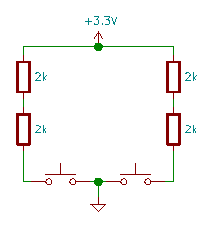
\includegraphics[height=37mm]{hw_final/buttons_circuit.eps}
%     %     %     \label{fig:matriz-hw-resto:botones_circuito}
%     %     % } \\
%     %     \subfigure[Base 3D]{
%     %         \includegraphics[height=75mm]{hw_final/3D_base.jpg}
%     %         \label{fig:matriz-hw-resto:base}
%     %     }
%     %     \caption{Matriz de figuras} 
%     %     \label{fig:matriz-hw-resto}
%     % \end{figure}
% % \end{enumerate}


% %!
% \subsection{Funcionalidades disponibles.}
% \begin{itemize}
%     \item Comunicación serie bidireccional con velocidad configurable de hasta 3750000bauds, f
%     \item s
% \end{itemize}


% %!
% \subsection{Simulación global previa.}
% Previamente al sintetizado y uso de la configuración de la \emph{FPGA}, se han realizado diversas pruebas que, por un lado, han ayudado a encontrar errores que puedan dañar los propios componentes \emph{hardware}, y por otro lado, a verificar el correcto funcionamiento de las funcionalidades de dicha configuración.

% % \noWord[Mover al capitulo de procediminetos??]\\
% % Tal como está explicado en el capítulo de procedimientos (Cap. \ref{ch:procedimiento}), para la simulación del código de \emph{Verilog} se utiliza \emph{Icarus Verilog} \footnote{Véase su repositorio: \url{https://github.com/steveicarus/iverilog}}, herramienta de código libre creada por Stephen Williams \footnote{Vease su página personal: \url{http://stevewilliams.icarus.com/}} capaz de simular es estandar de \emph{Verilog IEEE Std 1364-2005} \\
% % \noWord[Fin.]

% Tal como está explicado en el capítulo de procedimientos (Cap. \ref{ch:procedimiento}), para la simulación del código de \emph{Verilog} se utiliza la herramienta de código abierto \emph{Icarus Verilog} \footnote{Véase su repositorio: \url{https://github.com/steveicarus/iverilog}}, que junto con el visor de ondas \emph{GTKWave}, permiten generar y mostrar todas las señales del circuito en cualquier instante de tiempo.

% La simulación global, aun estando dentro del mismo archivo, se ha dividido en varias pruebas.
% \begin{enumerate}
%     %!
%     \item \textbf{Pruebas 1 y 2.} Reseteo y prueba de botones auxiliares. \\
%     as
    
%     %!
%     \item \textbf{Prueba 3.} Comando de lectura de registro. \\
%     as

%     %!
%     \item \textbf{Prueba 4.} Comando de transmisión del último registro leido. \\
%     as
    
%     %!
%     \item \textbf{Prueba 5.} Comando de escritura de registro. \\
%     as
    
%     %!
%     \item \textbf{Prueba 6.} Captación de 6 bytes \noWord[Añadir símbolo] USB. \\
%     as
    
%     %!
%     \item \textbf{Prueba 7.} Comando para empezar la transmisión de la captura al PC. \\
%     as
    
%     %!
%     \item \textbf{Prueba 8.} Captación de 4 bytes \noWord[Añadir símbolo] USB. \\
%     as
    
%     %!
%     \item \textbf{Prueba 9.} Captación de cambio de estado del bus USB. \\
%     as
    
%     %!
%     \item \textbf{Prueba 10.} Comando de finalización de transmisión de datos al PC. \\
%     as
% \end{enumerate}

% %!
% \subsection{sintetizado final \noWord[Cambiar titulo??]}


% %!
% \section{\emph{Software} de control.}


% \warning{viejo} \\
% %!
% En este capitulo se comentan los diversos resultados obtenidos en el presente TFG, tanto los relacionados con la \emph{FPGA} (\emph{Hardware} utilizado, simulaciones y sintetizado final), como con el \emph{Software} de control. Se incluyen además fotografiás que complementan lo explicado.

% %!
% \section{Componentes \emph{Hardware} utilizados}
% El sistema final del analizador USB está compuesto de las siguientes partes.
% \begin{enumerate}
%     \item \textbf{Placa de desarrollo \emph{IceStick \cite{icestickmanual}}.} \\
%     Placa de desarrollo que incorpora, sin contar con todos los conectores, elementos pasivos y componentes de regulación, la \emph{FPGA iCE40HX-1k \cite{lattice:ice40}} del fabricante \emph{Lattice}, memoria SPI de 32MBit para almacenar el sintetizado generado para la \emph{FPGA}, conversor USB a doble puerto de comunicación FIFO \emph{FTDI 2232H \cite{FTDI:FT2232HL}} y oscilador de $12MHz$ con el que referenciar ciertas partes del circuito.
%     \item \textbf{Placa de desarrollo \emph{USB3300 \cite{icestickmanual}}.} \\
%     Placa de desarrollo que incorporated.
% \end{enumerate}


% %!
% \section{Comparativa de precios}


% %!
% \section{Resultados de la simulación}
% Siguiendo los pasos establecidos en el capitulo de procedimientos (\ref{ch:procedimiento}) \noWord [ref a capitulo procedimientos], se realiza una simulación general en la que probar la mayor parte de las funcionalidades, intentando mantener las mismas características que el sistema final.


% %!
% \section{Resultados en la \emph{FPGA}}
% Tras asegurar
% \begin{enumerate}
%     \item Maxima velocidad estable del reloj.
%     \item ds
% \end{enumerate}

% %!
% \section{Resultados del \emph{software} de captación}
% % ###



% \chapter{Resultados}
% \label{ch:resultados_plantilla}

% Escribe en este capítulo los resultados del proyecto.  Este capítulo debería explicar los resultados de forma global, no los resultados de cada iteración.  Probablemente será el capítulo con más tablas y gráficas. Revisa las secciones~\ref{sec:figuras} y~\ref{sec:tablas} para aprender cómo se escriben en \LaTeX{}.